%%%%%%%%%%%%%%%%%%%%%%%%%%%%%%%%%%%%%%%%%%%%%%%%%%%%%%%%%%%%%%%%%%%%%%%%
\chapter{Le basi statistiche della termodinamica}
\label{cap:basi}
%%%%%%%%%%%%%%%%%%%%%%%%%%%%%%%%%%%%%%%%%%%%%%%%%%%%%%%%%%%%%%%%%%%%%%%%

%%%%%%%%%%%%%%%%%%%%%%%%%%%%%%%%%%%%%%%%%%%%%%%%%%%%%%%%%%%%%%%%%%%%%%%%
% MACROSTATO E MICROSTATI
%
\section{Macrostato e microstati}
\label{sec:02-microstati}
%%%%%%%%%%%%%%%%%%%%%%%%%%%%%%%%%%%%%%%%%%%%%%%%%%%%%%%%%%%%%%%%%%%%%%%%

Partiamo da considerazioni di carattere completamente generale e prendiamo in esame un sistema fisico macroscopico all'equilibrio, costituito da $N$ particelle identiche (atomi o molecole) confinate in un volume $V$. Considerando i valori tipici di $N$, che sono dell'ordine del numero di Avogadro, e il rapporto tra $V$ e le distanze atomiche tipiche, è naturale pensare al cosiddetto {\em limite termodinamico}: mandiamo cioè sia $N$ sia $V$ all'infinito ma in modo tale che il loro rapporto $n = N/V$, che rappresenta la densità numerica del sistema, resti costante (vedi la sezione \ref{sec1:def} del capitolo \ref{cap:termodinamica}). Per ottenere la vera densità sarà sufficiente moltiplicare $n$ per la massa $m$ delle particelle.

Per semplificare le cose immaginiamo che le particelle non interagiscano l'una con l'altra (questa situazione è l'idealizzazione di un sistema fisico in cui l'interazione tra i costituenti elementari può essere ritenuta, in prima approssimazione, trascurabile): in questo caso l'energia totale del sistema sarà semplicemente la somma delle energie delle singole particelle, e cioè
\be
\label{eq:etot}
E = \sum_{i} n_{i}\epsilon_{i}
\ee
in cui $\epsilon_{i}$ rappresenta l'energia (di singola particella) dell'$i$-mo livello, mentre $n_{i}$ è il numero di occupazione del livello stesso (ossia indica quante particelle occupano quel livello). Naturalmente il set $\seti{n_{i}}$ deve soddisfare il vincolo
\be
\label{eq:ntot}
N = \sum_{i} n_{i}
\ee

Poiché abbiamo a che fare con stati microscopici è naturale utilizzare il formalismo quantistico, e dato che il sistema è confinato nel volume $V$ i livelli di energia $\epsilon_{i}$ saranno discreti. Quindi anche $E$ assume valori discreti, ma dato lo stratosferico numero di livelli e la loro spaziatura fine possiamo considerare $E$, quando risulta comodo, come una variabile continua a tutti gli effetti pratici.

L'assegnazione della terna $(N,V,E)$ equivale a specificare un {\em macrostato} del sistema; se però consideriamo le cose dal punto di vista molecolare vediamo subito che esisteranno moltissimi modi diversi per ottenere lo stesso macrostato. Consideriamo il seguente sistema ipersemplificato, consistente in una cassettiera con tre cassetti ($V=3$) e $N$ biglie ($N = 10$). Se una biglia è nel primo cassetto in basso la sua energia vale $\epsilon_{1} = 0$, se è nel cassetto di centro abbiamo $\epsilon_{2} = 1$ (in certe unità), mentre se è nel cassetto superiore la sua energia è $\epsilon_{3} = 2$. Sappiamo che l'energia totale del sistema, nelle stesse unità energetiche di prima, vale $E = 10$. Avendo assegnato la terna $(N,V,E)$ abbiamo specificato un macrostato della cassettiera con biglie, e dal punto di vista microscopico possiamo realizzare lo stesso macrostato in modi diversi. Solo per fare qualche esempio, potremmo sistemare $3$ biglie nel cassetto superiore, $4$ in quello di mezzo e $3$ nel cassetto in basso, oppure $10$ biglie nel cassetto di mezzo, eccetera. Tutti questi diversi microstati realizzano un unico macrostato di equilibrio a energia fissata, e dovrebbe risultare chiaro che il numero dei microstati compatibili con il macrostato d'equilibrio sarà funzione di $N$, $V$, e $E$: abbiamo dunque $\Omega(N,V,E)$.

In linea del tutto generale i microstati possono essere identificati con le soluzioni indipendenti dell'equazione di Schr\"odinger che corrispondono all'autovalore $E$ dell'Hamiltoniana totale del sistema. Sembra abbastanza naturale assumere che a ogni tempo $t$ può stare con probabilità uguale in ciascun microstato, ovvero che ogni microstato è ugualmente probabile. Questo è noto come il {\em postulato di uguale probabilità a priori}, e si fonda sulla convinzione che se due microstati hanno la stessa energia il sistema non ha motivi particolari per preferire l'uno all'altro. 

%%%%%%%%%%%%%%%%%%%%%%%%%%%%%%%%%%%%%%%%%%%%%%%%%%%%%%%%%%%%%%%%%%%%%%%%
% PRIMO CONTATTO
%
\section{Primo contatto con la termodinamica}
\label{sec:primo}
%%%%%%%%%%%%%%%%%%%%%%%%%%%%%%%%%%%%%%%%%%%%%%%%%%%%%%%%%%%%%%%%%%%%%%%%

Consideriamo due sistemi fisici, $A_{1}$ e $A_{2}$, entrambi separatamente all'equilibrio. Il primo sistema è in un macrostato caratterizzato dai valori $(N_{1},V_{1},E_{1})$ e nel quale il numero di microstati è pari a $\Omega_{1}(N_{1},V_{1},E_{1})$, mentre il secondo dai valori $(N_{2},V_{2},E_{2})$ e da un numero di microstati pari a $\Omega_{2}(N_{2},V_{2},E_{2})$. Poniamo i due sistemi in contatto termico (vedi figura \ref{fig:a1a2}); ciò equivale a dire che i due sistemi possono ora scambiare energia termica tra di loro, a volume e numero di particelle fissati. Le energie dei due sistemi non saranno più uguali a $E_{1}$ e $E_{2}$, ma la loro somma rimarrà conservata: $E = E_{1} + E_{2}$ (stiamo trascurando l'energia di interazione tra $A_{1}$ e $A_{2}$, assumendola come un termine di superficie; ciò è sempre lecito nel limite termodinamico). Risulta chiaro, per definizione stessa di numero di microstati, che il valore di $\Omega$ per i due sistemi in contatto, considerati come un unico sistema, sarà pari a
\be
\label{eq:omega}
\Omega(E_{1}, E_{2}) = \Omega_{1}(E_{1})\Omega_{2}(E_{2}) = \Omega_{1}(E_{1})\Omega_{2}(E-E_{1}) \equiv \Omega(E,E_{1})
\ee
Ci si pone dunque la domanda: per quale valore di $E_{1}$ il sistema complessivo è in equilibrio?

%%%%%%%%%%%%%%%%%%%%%%%%%%%%%%%%%%%%%%%%%%%%%%%%%%%%%%%%%%%%%%%%%%%%%%
\begin{figure}[!ht]
  \centering
  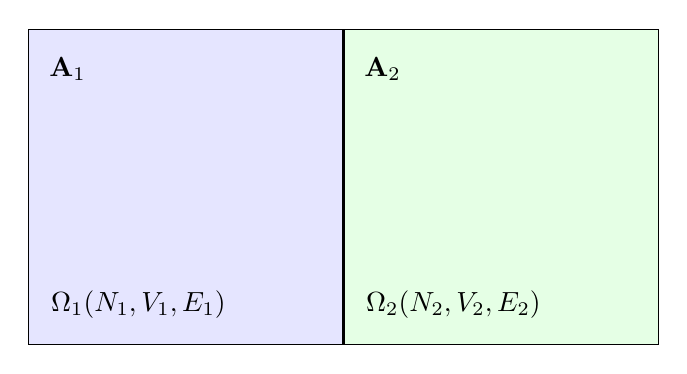
\begin{tikzpicture}
  \draw[fill=blue!10!white] (0,0)--(0,4)--(4,4)--(4,0)--(0,0);
  \draw[fill=green!10!white,xshift=4cm] (0,0)--(0,4)--(4,4)--(4,0)--(0,0);
  \draw[very thick] (4.0,0.0)--(4.0,4.0);
  \draw (0.5,3.5) node{$\mathbf{A}_1$};
  \draw (1.4,0.5) node{$\Omega_1(N_1, V_1, E_1)$};  
  \draw (0.5,3.5) [xshift=4cm] node{$\mathbf{A}_2$};
  \draw (1.4,0.5) [xshift=4cm] node{$\Omega_2(N_2, V_2, E_2)$};  
\end{tikzpicture}

  \caption{Due sistemi in contatto termico.}
  \label{fig:a1a2}
\end{figure}
%%%%%%%%%%%%%%%%%%%%%%%%%%%%%%%%%%%%%%%%%%%%%%%%%%%%%%%%%%%%%%%%%%%%%%

Sembra ragionevole pensare che ciò accada per un valore di $E_1$ che rende stazionaria $\Omega$; infatti se $\Omega$ non fosse stazionaria il sistema non sarebbe (ancora) all'equilibrio. Sembra anche ragionevole assumere che in realtà $E_{1}$ {\em massimizza} $\Omega$. L'idea che sta dietro quest'assunzione è che un sistema fisico fuori dall'equilibrio evolve naturalmente in una direzione che gli permette di assumere un numero sempre crescente di microstati, finché non arriva in un macrostato che permette il numero più grande possibile di microstati compatibili con il macrostato d'equilibrio; questo perché da un punto di vista statistico riteniamo che i macrostati con un numero maggiore di microstati possibili siano più probabili di quelli con un numero minore di microstati.

Chiamiamo dunque $\bar{E}_{1}$ il valore di $E_{1}$ per il quale il sistema totale è all'equilibrio (e quindi l'energia di $A_{2}$ sarà pari a $\bar{E}_{2}$) e scriviamo la condizione di massimo per $\Omega$:
\be
\label{eq:maxomega1}
\dparc{\Omega}{E_{1}}{E_{1}=\bar{E}_{1}} = \dparc{\Omega_{1}}{E_{1}}{E_{1}=\bar{E}_{1}}\Omega_{2}(\bar{E_{2}}) + \Omega_{1}(\bar{E}_{1})\dparc{\Omega_{2}}{E_{2}}{E_{2}=\bar{E}_{2}}\dpar{E_{2}}{E_{1}} = 0
\ee
Ma $\partial E_{2}/\partial E_{1} = -1$, e arriviamo quindi a
\be
\label{eq:maxomega2}
\dparc{\Omega_{1}}{E_{1}}{E_{1}=\bar{E}_{1}}\Omega_{2}(E_{2}) = \dparc{\Omega_{2}}{E_{2}}{E_{2}=\bar{E}_{2}}\Omega_{1}(\bar{E}_{1})
\ee
cioè
\be
\label{eq:maxomega3}
\dparc{\ln \Omega_{1} }{E_{1}}{E_{1}=\bar{E}_{1}} = 
\dparc{\ln \Omega_{2} }{E_{2}}{E_{2}=\bar{E}_{2}}
\ee
Definendo
\be
\label{eq:beta}
\beta_i \equiv \dpar{\ln \Omega_i }{E_i}
\ee
abbiamo che i due sistemi sono all'equilibrio quando $\beta_{1} = \beta_{2}$. Risulta chiaro che il parametro $\beta$ deve avere qualcosa a che fare con la temperatura, visto che la condizione per la quale due sistemi a contatto termico siano all'equilibrio è data proprio da $T_{1} = T_{2}$. Riprendendo le formule termodinamiche, ricordiamo che
\be
\label{eq:unosut}
\frac{1}{T} = \dparc{S}{E}{N,V}
\ee
e prendendo il rapporto tra la (\ref{eq:beta}) e la (\ref{eq:unosut}) per variazioni piccole ma {\em finite} di $S$ e $\ln{\Omega}$ otteniamo
\be
\label{eq:deltaomega}
\frac{\Delta S}{\Delta(\ln \Omega)} = \frac{1}{\beta T} = \mbox{costante}
\ee
Fu Boltzmann il primo a capire la relazione tra l'entropia e il numero dei microstati accessibili al sistema, anche se il primo a scrivere l'equazione che segue fu Planck:
\be
\label{eq:entropia}
S = k\ln \Omega
\ee
Questa formula è il ponte che collega il mondo microscopico (conteggio dei microstati) al mondo macroscopico (entropia). Occorre tenere presente che il risultato che abbiamo appena visto, sebbene corretto, è stato ottenuto con ragionamenti euristici, non esattamente rigorosi. In quel che segue daremo per scontato che l'entropia è definita dall'eq. (\ref{eq:entropia}); vedi anche l'esercizio \ref{ex2:relaSOmega}.

%%%%%%%%%%%%%%%%%%%%%%%%%%%%%%%%%%%%%%%%%%%%%%%%%%%%%%%%%%%%%%%%%%%%%%
\subsection{Volume e pressione}
%%%%%%%%%%%%%%%%%%%%%%%%%%%%%%%%%%%%%%%%%%%%%%%%%%%%%%%%%%%%%%%%%%%%%%

Possiamo pensare che la parete divisoria che separa $A_{1}$ e $A_{2}$ sia fatta in modo tale da scorrere e permettere un cambiamento dei volumi $V_{1}$ e $V_{2}$. Ripetendo il ragionamento fatto prima a proposito dell'energia, arriviamo al risultato che all'equilibrio (meccanico oltre che termico) deve valere la relazione
\be
\label{eq:omegavolume}
\dpar{\ln \Omega_{1}}{V_{1}} = 
\dpar{\ln \Omega_{2}}{V_{2}}
\ee
Definiamo quindi un nuovo parametro
\be
\eta \equiv \dparc{\ln \Omega}{V}{N,E}
\ee
in cui abbiamo esplicitato il fatto che la derivata rispetto a $V$ va fatta tenendo costanti sia $N$ sia $E$. Per capire il significato fisico di $\eta$ torniamo alla prima legge della termodinamica:
\be
\de{E} = T\de{S} - P\de{V}
\ee
e considerando $E$ costante otteniamo
\be
T\dparc{S}{V}{E} = P
\ee
Otteniamo quindi subito
\be
\label{eq:eta}
\eta = \frac{P}{kT}
\ee
Questo risultato è abbastanza ovvio, perché è chiaro che il sistema $A_{1}+A_{2}$ è all'equilibrio sia termico sia meccanico quando le temperature e le pressioni nei due scomparti sono uguali.

%%%%%%%%%%%%%%%%%%%%%%%%%%%%%%%%%%%%%%%%%%%%%%%%%%%%%%%%%%%%%%%%%%%%%%
\subsection{Il potenziale chimico}
%%%%%%%%%%%%%%%%%%%%%%%%%%%%%%%%%%%%%%%%%%%%%%%%%%%%%%%%%%%%%%%%%%%%%%

Assumiamo ora che la parete divisoria sia porosa, in modo tale da permettere il passaggio degli atomi dalla partizione $A_1$ a quella $A_2$ e viceversa. Quindi ora anche $N_1$ ed $N_2$ possono variare. Ripetendo i ragionamenti già svolti e definendo
\be
\zeta_i \equiv \dparc{\ln \Omega_i}{N_i}{V,E}
\ee
abbiamo che all'equilibrio deve valere
\be
\zeta_1 = \zeta_2 = \zeta
\ee
Scrivendo la forma completa del primo principio della termodinamica,
\be
\de E = T\de S - P\de V + \mu\de N
\ee
otteniamo subito
\be
\zeta = -\frac{\mu}{kT}
\ee
e quindi la condizione di equilibrio
\be
\mu_1 = \mu_2
\ee

%%%%%%%%%%%%%%%%%%%%%%%%%%%%%%%%%%%%%%%%%%%%%%%%%%%%%%%%%%%%%%%%%%%%%%
\section{Il gas ideale}
%%%%%%%%%%%%%%%%%%%%%%%%%%%%%%%%%%%%%%%%%%%%%%%%%%%%%%%%%%%%%%%%%%%%%%

Anche senza calcolare $\Omega$ possiamo già ottenere qualche risultato. Consideriamo per esempio un gas ideale monoatomico. Poiché gli atomi del gas sono considerati come non--interagenti non c'è alcuna correlazione tra le posizioni delle particelle, e quindi il numero possibile di modi in cui possono essere distribuite $N$ particelle sarà uguale al prodotto (su tutte le particelle) del numero di modi in cui ogni particella può disporsi. Per una singola particella, a energia fissata, avremo che questo numero dovrà necessariamente essere proporzionale al volume $V$, e otteniamo dunque
\be
\Omega \propto V^{N}
\ee
Ma dalla (\ref{eq:eta}) abbiamo
\be
\frac{P}{kT} = \dpar{\ln \Omega}{V} = \frac{N}{V}
\ee
e riconosciamo subito l'equazione di stato del gas ideale:
\be
PV = NkT
\ee
Per ottenere più informazioni sarà il caso di conoscere meglio $\Omega$.

%%%%%%%%%%%%%%%%%%%%%%%%%%%%%%%%%%%%%%%%%%%%%%%%%%%%%%%%%%%%%%%%%%%%%%
\subsection{Particelle in una scatola}
%%%%%%%%%%%%%%%%%%%%%%%%%%%%%%%%%%%%%%%%%%%%%%%%%%%%%%%%%%%%%%%%%%%%%%

Formalizziamo la situazione nel modo seguente: abbiamo un sistema fisico (gas ideale, particelle non interagenti) racchiuso in una scatola di dimensioni lineari $L$ (con $L^{3}=V$). Sia $\epsilon_{i}$ il valore dell'$i$-mo livello di energia di singola particella, e sia $n_{i}$ il numero di occupazione del livello (ossia quante particelle vengono ospitate in quel livello). Abbiamo dunque
\bea
\label{eq:vincoli}
N &=& \sum_{i} n_{i}\nonumber\\
E &=& \sum_{i} n_{i}\epsilon_{i}
\eea
Vogliamo sapere in quanti modi possiamo sistemare le $N$ particelle nei livelli in modo tale da soddisfare {\em contemporaneamente} i vincoli (\ref{eq:vincoli}). Come prima cosa converrà ricordare la formula per l'energia di una particella di massa $m$ in una scatola con condizioni al bordo $\psi=0$ (potenziale infinito):
\be
\label{eq:livelliscatola}
\epsilon(n_{x},n_{y},n_{z}) = \frac{h^{2}}{8mL^{2}}(n^{2}_{x} + n^{2}_{y} + n^{2}_{z})\quad n_{x},n_{y},n_{z} = 1, 2, 3\dots
\ee
Quindi per {\em una} particella di energia $\epsilon$ il numero di {\em autofunzioni distinte} (ovvero microstati) è pari al numero di soluzioni intere e positive dell'equazione
\be
n^{2}_{x} + n^{2}_{y} + n^{2}_{z} = \frac{8mV^{2/3}\epsilon}{h^{2}} \equiv \epsilon^{*}
\ee
e più in generale il valore di $\Omega$ sarà dato dal numero delle soluzioni intere e positive di
\be
\label{eq:estar}
\sum_{r=1}^{3N}n^{2}_{r} = \frac{8mV^{2/3}E}{h^{2}} \equiv E^{*}
\ee
Dall'equazione precedente possiamo ricavare un altro risultato importante senza calcolare $\Omega$; vediamo infatti che in ogni caso $\Omega$ non dipende da $V$ e da $E$ separatamente ma solo tramite la combinazione $V^{2/3}E$, e questo si rifletterà sulla dipendenza da $E$ e $V$ dell'entropia:
\be
S(N,V,E) \equiv S(N,V^{2/3}E)
\ee
Per un processo adiabatico abbiamo $S = \mbox{costante}$ e quindi $V^{2/3}E = \mbox{costante}$. Usando la (\ref{eq:beta}) e la (\ref{eq:eta}) possiamo scrivere
\be
P = \dparc{S}{V}{E} \big{/} \dparc{S}{E}{V} = \dparc{S}{V}{E}\dparc{E}{S}{V}
\ee
Ma se tre grandezze $x$, $y$ e $z$ sono legate da una relazione funzionale, allora abbiamo che
\be
\label{eq:02-magic2}
\dparc{x}{y}{z}\dparc{y}{z}{x}\dparc{z}{x}{y} = -1
\ee
e possiamo dunque scrivere
\be
P = -\dparc{E}{V}{S} = \frac{2}{3}\frac{E}{V}
\ee
e quindi, sostituendo nell'espressione $V^{2/3}E = \mbox{costante}$ otteniamo proprio l'equazione per una trasformazione adiabatica:
\be
PV^{\gamma} = \mbox{costante}\quad\quad \gamma=5/3
\ee
È da notare che questi risultati valgono sia in ambito classico sia in ambito quantistico, perché non abbiamo nemmeno ancora calcolato il valore di $\Omega$.

%%%%%%%%%%%%%%%%%%%%%%%%%%%%%%%%%%%%%%%%%%%%%%%%%%%%%%%%%%%%%%%%%%%%%%
\subsection{Il calcolo di $\Omega$}
%%%%%%%%%%%%%%%%%%%%%%%%%%%%%%%%%%%%%%%%%%%%%%%%%%%%%%%%%%%%%%%%%%%%%%

Calcoliamo $\Omega(E^{*})$ assumendo che le particelle siano {\em distinguibili}, altrimenti il conto risulta troppo difficile. $\Omega(E^{*})$ sarà uguale al numero di punti di un reticolo $3N$--dimensionale (in cui le coordinate dei siti sono etichettate da numeri interi) che giacciono sulla superficie di un'ipersfera di raggio $\sqrt{E^{*}}$. Per chiarire le idee prendiamo un esempio bidimensionale (vedi figura \ref{fig:e25}). Poniamo conto che sia $E^{*} = 25$ (in certe unità). L'equazione $n^{2}_{1} + n^{2}_{2} = E^{*}$ è risolta dai punti $(3,4)$ e $(4,3)$ e abbiamo dunque due soluzioni.

Dovrebbe risultare chiaro che in generale, nel caso $3N$--dimensionale, $\Omega$ sarà una funzione estremamente irregolare di $E^{*}$, perché cambiamenti molto piccoli di $E^{*}$ possono causare una grande fluttuazione nel numero di punti che giacciono {\em esattamente} sulla superficie dell'ipersfera. Invece di considerare $\Omega$ consideriamo al suo posto la quantità
\be
\label{eq:sigma}
\Sigma_{N}(E^{*}) = \sum_{E'\le E^{*}}\Omega(E')
\ee
ovvero consideriamo tutti i punti che cadono all'interno del volume dell'ipersfera, nella speranza che questa nuova funzione sia un po' meno irregolare di $\Omega$. Vedremo poi in dettaglio il perché di questa scelta. Per il momento diremo solo, postponendo la spiegazione, che per trovare l'entropia il calcolo di $\Sigma_{N}$ è equivalente a quello di $\Omega$.

%%%%%%%%%%%%%%%%%%%%%%%%%%%%%%%%%%%%%%%%%%%%%%%%%%%%%%%%%%%%%%%%%%%%%%
\begin{figure}[!ht]
  \centering
  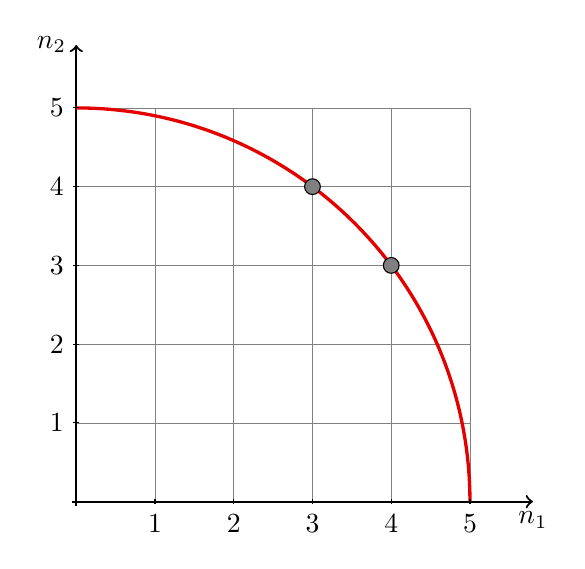
\begin{tikzpicture}
  \draw[step=1,gray,very thin] (0.0,0.0) grid (5.0,5.0);
  \draw[->=Stealth,thick] (-0.05,0.0)--(5.8,0.0) node[anchor=north]{$n_1$};
  \draw[->=Stealth,thick] (0.0,-0.05)--(0.0,5.8) node[anchor=east]{$n_2$};
  \draw[color=red!90!black,very thick] (5,0) arc [start angle=0, end angle=90, radius=5];
  
  \draw[fill=gray] (3,4) circle (0.1);
  \draw[fill=gray] (4,3) circle (0.1);

  \foreach \x in {1,...,5}
    \draw (\x cm,1pt) -- (\x cm,-1pt) node[anchor=north] {$\x$};
  \foreach \y in {1,...,5}
    \draw (1pt,\y cm) -- (-1pt,\y cm) node[anchor=east] {$\y$};
\end{tikzpicture}

  \caption{Le due soluzioni dell'esempio bidimensionale proposto nel testo.}
  \label{fig:e25}
\end{figure}
%%%%%%%%%%%%%%%%%%%%%%%%%%%%%%%%%%%%%%%%%%%%%%%%%%%%%%%%%%%%%%%%%%%%%%

Il numero di punti all'interno del volume sarà {\em asintoticamente} uguale al volume dell'iper--ottante positivo di una sfera in $3N$ dimensioni di raggio $\sqrt{E^{*}}$.

%%%%%%%%%%%%%%%%%%%%%%%%%%%%%%%%%%%%%%%%%%%%%%%%%%%%%%%%%%%%%%%%%%%%%%
\subsection{Volume e superficie di una sfera in $n$ dimensioni}
%%%%%%%%%%%%%%%%%%%%%%%%%%%%%%%%%%%%%%%%%%%%%%%%%%%%%%%%%%%%%%%%%%%%%%

In $n$ dimensioni scriviamo l'elemento di volume come
\be
\de{V_{n}} = \prod_{i=1}^{n}\de{x_{i}}
\ee
e ci proponiamo di calcolare il volume dell'ipersfera di raggio $R$:
\be
V_{n}(R) = \int \cdots \int\limits_{0\le\sum_{i=1}^{n}x^{2}_{i}\le R^{2}}\de{V_{n}}
\ee
È chiaro che $V_{n}(R)$ sarà proporzionale a $R^{n}$, e scriviamo quindi $V_{n}(R) = C_{n}R^{n}$, in cui $C_{n}$ è un coefficiente che non dipende più da $R$. Abbiamo quindi un'espressione alternativa per la misura:
\be
\de{V_{n}} = nC_{n}R^{n-1}\de{R}
\ee
Inoltre possiamo sempre scrivere $\de{V_{n}} = S_{n}(R)\de{R}$, in cui $S_{n}(R)$ è la superficie dell'ipersfera, e dal confronto con la precedente ricaviamo
\be
S_{n}(R) = nC_{n}R^{n-1}
\ee
Partiamo ora dal semplice integrale gaussiano:
\be
\int_{-\infty}^{\infty}e^{-x^{2}}\de{x} = \pi^{1/2}
\ee
ed elevando entrambi i membri alla potenza $n$ otteniamo:
\be
\pi^{n/2} = \int\cdots\int\limits_{-\infty<x_{i}<\infty} \exp\left(\sum_{i}x^{2}_{i}\right)\prod_{i}\de{x_{i}} = \int_{0}^{\infty} e^{-R^{2}} nC_{n}R^{n-1}\de{R}
\ee
Utilizziamo ora il risultato (valido per $\nu > -1$) per un integrale gaussiano generalizzato:
\be
I_{\nu}(\alpha) = \int_{0}^{\infty}\de{y}\;y^{\nu}e^{-\alpha y^{2}} = \frac{1}{2\alpha^{(\nu+1)/2}}\Gamma\bfrac{\nu+1}{2}
\ee
e sostituiamo i valori rilevanti per il nostro caso: $\alpha = 1$, $\nu = n-1$, e otteniamo
\be
\pi^{n/2} = C_{n}\frac{n}{2}\Gamma\bfrac{n}{2} = C_{n}\bfrac{n}{2}!
\ee
in cui nell'ultimo passaggio abbiamo sfruttato le proprietà della funzione $\Gamma$:
\be
\Gamma(n+1) = n\Gamma(n) = n! 
\ee
Per la definizione della funzione $\Gamma$ vedi la sottosezione \ref{subsec:app1-gamma} dell'appendice \ref{app:matematica}. Otteniamo quindi
\be
C_{n} = \pi^{n/2} {\big/} \bfrac{n}{2}!
\ee
e in definitiva le formule che ci interessano:
\bea
S_{n}(R) &=& \frac{2\pi^{n/2}}{\Gamma(n/2)}R^{n-1}\nonumber\\
V_{n}(R) &=& \frac{\pi^{n/2}}{(n/2)!}R^{n}
\eea

%%%%%%%%%%%%%%%%%%%%%%%%%%%%%%%%%%%%%%%%%%%%%%%%%%%%%%%%%%%%%%%%%%%%%%
\subsection{Continua il calcolo di $\Omega$}
%%%%%%%%%%%%%%%%%%%%%%%%%%%%%%%%%%%%%%%%%%%%%%%%%%%%%%%%%%%%%%%%%%%%%%

Applicando la formula per il volume dell'ipersfera al nostro caso otteniamo
\be
\Sigma_{N}(E^{*}) \simeq \frac{1}{2^{3N}}\left[\frac{\pi^{3N/2}}{(3N/2)!}E^{* 3N/2} \right]
\ee
(il fattore $1/2^{3N}$ deriva dal fattore $1/8$ per ogni particella, perché stiamo considerando solo un ottante dell'ipersfera). Sostituendo a $E^{*}$ il suo valore dato dall'equazione (\ref{eq:estar}) otteniamo
\be
\Sigma_{N}(E,V) \simeq \bfrac{V}{h^{3}}^{N}\frac{(2\pi mE)^{3N/2}}{(3N/2)!}
\ee
Prendiamo il logaritmo di quest'ultima espressione e applichiamo la fomula di Stirling (vedi la sottosezione \ref{subsec:app1-stirling} dell'appendice \ref{app:matematica}, valida nel limite in cui $n$ va a infinito:
\be
\ln(n!) = n\ln n - n + \dots
\ee

%%%%%%%%%%%%%%%%%%%%%%%%%%%%%%%%%%%%%%%%%%%%%%%%%%%%%%%%%%%%%%%%%%%%%%
\begin{Nota}
\`E da notare che sebbene valga per valori asintotici di $n$, già per $n=20$ la formula di Stirling restituisce il valore del $\ln(n!)$ con un errore relativo di circa lo $0.6\%$.
\end{Nota}
%%%%%%%%%%%%%%%%%%%%%%%%%%%%%%%%%%%%%%%%%%%%%%%%%%%%%%%%%%%%%%%%%%%%%%

Abbiamo dunque
\be
\ln\left[ \bfrac{V}{h^{3}}^{N}\frac{(2\pi mE)^{3N/2}}{(3N/2)!} \right] \simeq N\ln\left[\bfrac{V}{h^{3}}\bfrac{4\pi mE}{3N}^{3/2}\right] + \frac{3N}{2}
\ee
Vogliamo ora arrivare a un risultato che abbiamo annunciato, ossia che per calcolare l'entropia possiamo servirci indifferentemente di $\Omega$ o di $\Sigma$. Per dimostrare questo risultato dobbiamo ammettere che il calcolo stesso di $\Omega$ è abbastanza insensato, perché occorrerebbe fissare {\em esattamente} il valore dell'energia. Ammettiamo invece (e la nostra assunzione è fisicamente giustificata, perché nessun sistema è perfettamente isolato dal resto dell'universo) che l'energia possa variare (o fluttuare) di una quantità $\Delta$ intorno a $E$, ossia che l'energia del sistema vari nell'intervallo $(E-\Delta/2,E+\Delta/2)$, con la condizione $\Delta \ll E$. Scegliamo $\Delta$ in modo tale che $\Delta/E \sim O(N^{-1/2})$: la giustificazione per questa scelta verrà data più tardi.

Calcoliamo dunque il numero $\Gamma$ di microstati in un guscio centrato intorno al valore $E$:
\be
\Gamma(N,E,V;\Delta) = \Sigma_{N}(N,V,E+\Delta/2) - \Sigma_{N}(N,V,E-\Delta/2) \simeq \dpar{\Sigma}{E}\Delta
\ee
e con un semplice calcolo otteniamo
\be
\Gamma(N,E,V;\Delta) \simeq \frac{3N\Delta}{2E}\Sigma(N,V,E)
\ee
oppure, in forma logaritmica
\bea
\ln[\Gamma(N,E,V;\Delta)] &=& N\ln\left[\bfrac{V}{h^{3}}\bfrac{4\pi mE}{3N}^{3/2}\right] + \frac{3N}{2}\nonumber\\
  &+& \left\{ \ln\bfrac{3N}{2} + \ln\bfrac{\Delta}{E}\right\}
\eea
I termini fra parentesi graffe nell'espressione che precede sono trascurabili nel limite termodinamico: il primo perché $\ln(N)/N \to 0$ quando $N\to\infty$, e il secondo per lo stesso motivo, perché a causa della nostra scelta di $\Delta$ è ancora un termine $O(\ln N )$.

A questo punto occorre notare che la scelta di $\Delta$ deve essere {\em ragionevole}. Non avremmo potuto scegliere $\Delta$ che va a zero nel limite in cui $N$ va a infinito, altrimenti il termine $\ln(\Delta/E)$ avrebbe comportato una divergenza.

Il risultato sorprendente è dunque che a tutti gli effetti pratici abbiamo
\be
\ln\Gamma \simeq \ln\Sigma
\ee
e cioè, detto in parole semplici, che il logaritmo del volume di un'iperarancia $N$--dimensionale è uguale al volume della sua iperbuccia, comunque scegliamo spessa la buccia (il risultato per $\Gamma$ non dipende da $\Delta$). Il motivo di questo sorprendente risultato risiede nel fatto che il tasso di crescita con $E$ del numero dei microstati ($E^{3N/2}$) è così enorme che anche contando {\em tutti} i microstati con energia compresa tra zero ed $E$ sono solo le {\em immediate vicinanze} di $E$ a dare il contributo dominante. Per il calcolo dell'entropia possiamo dunque utilizzare indifferentemente $\Gamma$ o $\Sigma$, ottenendo comunque il risultato
\be
S(N,V,E) = Nk\ln\left[ \frac{V}{h^{3}}\bfrac{4\pi mE}{3N}^{3/2}\right] + \frac{3}{2}Nk
\ee
e invertendo questa espressione otteniamo l'energia in funzione dell'entropia:
\be
E(N,V,S) = \frac{3h^{2}N}{4\pi mV^{2/3}}\exp\left( \frac{2S}{3Nk} - 1\right)
\ee
Con un'espressione esplicita per l'entropia possiamo recuperare sostanzialmente tutta la termodinamica del gas ideale. Calcoliamo prima di tutto la temperatura d'equilibrio del sistema tramite la relazione
\be
T = \dparc{E}{S}{N,V} = \frac{2E}{3Nk}
\ee
cioè la ben nota relazione tra energia e temperatura:
\be
E = \frac{3}{2}NkT
\ee
dalla quale discende subito
\be
C_{V} = \dparc{E}{T}{N,V} = \frac{3}{2}Nk \quad\quad C_{P} = \dparc{(E+PV)}{T}{N,P} = \frac{5}{2}Nk
\ee
in cui nell'ultima abbiamo usato le relazioni $E = (3/2)PV$ e $PV = NkT$.

%%%%%%%%%%%%%%%%%%%%%%%%%%%%%%%%%%%%%%%%%%%%%%%%%%%%%%%%%%%%%%%%%%%%%%
\section{Entropia di mescolamento e paradosso di Gibbs}
%%%%%%%%%%%%%%%%%%%%%%%%%%%%%%%%%%%%%%%%%%%%%%%%%%%%%%%%%%%%%%%%%%%%%%

C'è ancora qualcosa che non va: l'entropia che abbiamo appena calcolato non soddisfa il requisito di essere una quantità {\em estensiva}. Se fosse estensiva (come deve) allora moltiplicando per un fattore $\alpha$ tutte le grandezze estensive da cui dipende, lasciando dunque invariate le quantità intensive, si dovrebbe avere la trasformazione $S \to \alpha S$. Troviamo invece
\be
S(\alpha N, \alpha V, \alpha E) = \alpha Nk \left[ \ln(\alpha VC) + \frac{3}{2} \right] \ne \alpha S(N,V,E)
\ee
(in cui $C$ è una costante facile da identificare). Vediamo subito che il termine che crea il problema è il $\ln V$. Se l'entropia non fosse una quantità estensiva ciò vorrebbe dire che l'entropia di un sistema sarebbe diversa dalla somma delle entropie delle sue parti, il che è fisicamente inaccettabile.

Questo problema può essere visto ancora meglio (e vedere i problemi sotto la giusta luce spesso aiuta a risolverli) esaminando il così detto {\em paradosso di Gibbs}. Consideriamo due gas ideali {\em diversi} all'equilibrio e in contatto termico, quindi alla stessa temperatura $T$.

All'inizio abbiamo, per le entropie dei due sistemi, separatamente ($i = 1, 2$):
\be
S_{i} = N_{i}k\ln V_{i} + \frac{3}{2}N_{i}k\left[ 1 + \ln\left( \frac{4\pi m_{i}E_{i}}{3N_{i}h^{2}} \right) \right]
\ee
ma $2E_{i}/(3N_{i}) = kT$ per tutti e due i sistemi, e quindi
\be
S_{i} = N_{i}k\ln V_{i} + \frac{3}{2}N_{i}k\left[ 1 + \ln\left( \frac{2\pi m_{i}kT}{h^{2}} \right) \right]
\ee
Ora lasciamo che i gas si mescolino, rimuovendo la parete che li divide. L'entropia totale, dopo che il sistema ha raggiunto l'equilibrio, sarà
\be
S_{T} = \sum_{i=1}^{2}\left\{ N_{i}k\ln V + \frac{3}{2}N_{i}k\left[ 1 + \ln\bfrac{2\pi m_{i}kT}{h^{2}}\right] \right\}
\ee
in cui $V = V_{1} + V_{2}$. Calcoliamo la variazione di entropia $(\delta S)$ ({\em entropia di mescolamento}):
\be
(\delta S) = S_{T} - \sum_{i=1}^{2}S_{i} = k\left[ N_{1}\ln\bfrac{V_{1}+V_{2}}{V_{1}} + N_{2}\ln\bfrac{V_{1}+V_{2}}{V_{2}} \right]
\ee
Notiamo subito che c'è un incremento di entropia, perché $(\delta S) > 0$, e ciò è cosa buona e giusta perché abbiamo appena assistito a un processo {\em irreversibile} (dopo aver ottenuto un cappuccino sarà ben difficile tornare a un puro espresso e a un bicchier di latte semplicemente facendo al contrario i passi che hanno portato al cappuccino).

Nel caso speciale in cui $N_{1}/V_{1} = N_{2}/V_{2} = \rho$ (densità uguali, oltre alla temperatura) abbiamo
\be
(\delta S)^{*} = k\left[ N_{1}\ln\bfrac{N_{1}+N_{2}}{N_{1}} + N_{2}\ln\bfrac{N_{1}+N_{2}}{N_{2}} \right]
\ee
e abbiamo ancora, giustamente, $(\delta S)^{*} > 0$. Fin qui nessun problema.

Vediamo però cosa succede se nella procedura di mescolamento utilizziamo lo {\em stesso} gas in tutti e due i compartimenti (naturalmente avremo $m_{1} = m_{2} = m$). {\em Prima} del mescolamento la situazione è identica alla precedente. {\em Dopo} il mescolamento avremo
\be
S_{T} = N\ln V + \frac{3}{2}Nk\left[ 1 + \ln\bfrac{2\pi mkT}{h^{2}}\right]
\ee
con $N = N_{1} + N_{2}$; quest'espressione è identica alla precedente, e quindi anche l'entropia di mescolamento, se le densità iniziali sono uguali, è la medesima. 

Ma questo è un risultato paradossale, per il semplice motivo che il mescolamento di due porzioni dello {\em stesso} gas, porzioni che sono alla {\em stessa} densità, è un processo chiaramente {\em reversibile}: banalmente, basta rimettere al suo posto la parete divisoria e torniamo alla situazione di partenza; quindi la variazione di entropia dovrebbe essere esattamente zero.

Naturalmente c'è il trucco, e adesso lo sveliamo: se rimettiamo al suo posto la parete divisoria la situazione torna identica a quella di partenza {\em se e solo se} le particelle sono {\em indistinguibili}. L'unica cosa che conta è il loro numero, non il loro nome. In altre parole se fosse possibile etichettare gli atomi del gas allo stesso modo in cui etichettiamo le bocce del biliardo la configurazione in cui la famigerata boccia \textbf{8} è nel contenitore di sinistra e quella \textbf{15} nel contenitore di destra sarebbe {\em diversa} dalla configurazione in cui la posizione delle due bocce è intercambiata. Ma non possiamo dare un nome agli atomi, pena l'immediata confusione dei sensi e della matematica. Ciò che c'è di intrinsecamente {\em sbagliato} nel modo in cui abbiamo calcolato l'entropia è che abbiamo considerato le particelle come se fossero {\em distinguibili}. Abbiamo considerato le cose come se potessimo dare un nome alle particelle del gas, nella speranza di una risposta in caso di chiamata: purtroppo la materia, almeno nella sua configurazione di base\footnote{Al contrario stati altamente organizzati della materia possono arrivare all'abiezione di raccontarci i loro sogni, se non li si ferma prima.}, oltre che sorda e cieca è anche muta.

Per uscire dal paradosso in maniera {\em pulita} occorrerebbe un conteggio degli stati che tenga conto dell'indistinguibilità\footnote{La pronuncia corretta al primo tentativo di questa parola comporta un punto in più all'esame, in caso.} degli atomi che costituiscono il gas. Questo avverrà più tardi. Per il momento contiamo di cavarcela nello stesso modo in cui se l'è cavata a suo tempo Gibbs, ossia usando la formula di Stirling al contrario.

La proposta è questa: dividiamo il numero dei microstati per un fattore {\em ad hoc} pari a $1/N!$, e proviamo a rifare i conti. Otteniamo
\be
S(N,V,E) = Nk\ln\bfrac{V}{N} + \frac{3}{2}Nk\left[ \frac{5}{3} + \ln\bfrac{2\pi m kT}{h^{2}} \right]
\ee
Se mescoliamo due gas {\em diversi} ritroviamo l'espressione corretta, che abbiamo già calcolato. Ma se mescoliamo lo {\em stesso} gas otteniamo
\be
(\delta S) = k\left[ (N_{1}+N_{2})\ln\bfrac{V_{1}+V_{2}}{N_{1}+N_{2}} - N_{1}\ln\bfrac{V_{1}}{N_{1}} - N_{2}\ln\bfrac{V_{2}}{N_{2}} \right]
\ee
Se le densità sono le stesse otteniamo $(\delta S)^{*} = 0$, com'è lecito attendersi. Inoltre è facile vedere che con la prescrizione di Gibbs l'entropia e l'energia diventano vere quantità estensive. Gli altri risultati termodinamici che abbiamo ricavato restano inalterati.

Scriviamo l'energia in funzione dell'entropia:
\be
\label{eq:efs}
E(N,V,S) = \frac{3h^2N^{5/3}}{4\pi mV^{2/3}}\exp\left(\frac{2S}{3Nk}-\frac{5}{3}\right)
\ee
e deriviamo quest'espressione rispetto a $N$, a $V$ e $S$ costanti, per ottenere il potenziale chimico del gas ideale:
\be
\label{eq:mudef}
\mu = \dparc{E}{N}{V,S} = \frac{E}{N}\left(\frac{5}{3}-\frac{2S}{3Nk}\right)
\ee
Ora, ricordando che $E = 3NkT/2$ e che $PV = 2E/3$, otteniamo facilmente questo importante risultato:
\be
\label{eq:muG}
\mu N = \frac{5E}{3} - TS = E + PV - TS = G
\ee
In parole povere, $\mu$ corrisponde all'energia libera di Gibbs per particella. Da notare che un'entropia non additiva avrebbe portato a un risultato sbagliato per il potenziale chimico $\mu$ (vedi per esempio l'esercizio \ref{ex2:Saddit}).

%%%%%%%%%%%%%%%%%%%%%%%%%%%%%%%%%%%%%%%%%%%%%%%%%%%%%%%%%%%%%%%%%%%%%%%%
\section{La numerazione corretta dei microstati}
%%%%%%%%%%%%%%%%%%%%%%%%%%%%%%%%%%%%%%%%%%%%%%%%%%%%%%%%%%%%%%%%%%%%%%%%

Il paradosso di Gibbs nasce dal fatto che abbiamo calcolato il numero di microstati considerando i costituenti elementari del sistema macroscopico come distinguibili. L'abbiamo fatto in ragione di un principio di economia, perché altrimenti il calcolo sarebbe stato di gran lunga più complicato; in ogni caso abbiamo commesso un errore. Di fatto non sapremo mai se la particella $k$--esima sta nel livello $\epsilon_{i}$ al posto della particella $l$--esima che sta nel livello $\epsilon_{j}$. Non potremmo mai venire a conoscere l'eventuale azione di un qualche diavoletto che le scambi di posto. Tutto ciò che possiamo ragionevolmente sperare di sapere è il {\em numero} di particelle nello stato $i$ o nello stato $j$ (cioè ciò che sappiamo è ciò che in un modo o nell'altro possiamo misurare).

Il modo corretto di contare i microstati è quello di considerare la distribuzione $\{n_{i}\}$, cioè il numero di modi in cui $N$ particelle indistinguibili possono distribuirsi tra i vari livelli in modo tale da determinare un valore prefissato dell'energia $E$, e due microstati che differiscono per il mero scambio di particelle devono essere a tutti gli effetti considerati come lo stesso microstato.

Il numero totale di permutazioni tra $N$ particelle, per un dato e fissato set $\{n_{i}\}$, è
\be
W\{n\} = \frac{N!}{n_{1}!n_{2}!\dots n_{i}!\dots}
\ee
e quindi vediamo subito che la ricetta di Gibbs corregge il problema in maniera {\em grossolana}, perché corrisponde a cancellare solo il numeratore $N!$ e trascura quindi il dettaglio della distribuzione tra i vari livelli. C'è quindi da chiedersi perché la correzione di Gibbs tutto sommato funzioni, nonostante il fattore {\em spurio} del denominatore.

Da un punto di vista puramente {\em matematico} la prescrizione di Gibbs funziona se tutti gli $n_{i}!$ valgono {\em al massimo} $1$, cioè se il livello $i$-esimo di energia in media non è occupato, o è occupato pochissimo. Da un punto di vista fisico è chiaro che questa condizione può verificarsi quando il numero di livelli di energia accessibili al sistema in maniera sostanzialmente equiprobabile è molto maggiore del numero di particelle: in questo caso abbiamo che la maggior parte dei livelli ha numero di occupazione zero, e la probabilità che un livello sia occupato da più di una particella è molto piccola. Si vede subito che questa situazione corrisponde a un sistema {\em classico}, in condizioni di bassa densità e alta temperatura. Quando studieremo un sistema in regime quantistico, o ad alte densità, o a basse temperature, sarà giocoforza contare i microstati in maniera corretta; inoltre troveremo una condizione quantitativa che ci permetterà di capire se un sistema può essere considerato in regime classico oppure no.

%%%%%%%%%%%%%%%%%%%%%%%%%%%%%%%%%%%%%%%%%%%%%%%%%%%%%%%%%%%%%%%%%%%%%%
\section{Esercizi per il Capitolo \ref{cap:basi}}
%%%%%%%%%%%%%%%%%%%%%%%%%%%%%%%%%%%%%%%%%%%%%%%%%%%%%%%%%%%%%%%%%%%%%%

\begin{Exercise}[label={ex2:relaSOmega}, title={Relazione funzionale tra entropia e numero di microstati}]
Assumendo che l'entropia $S$ di un sistema fisico (con $E$, $N$ e $V$ fissati) sia collegata al numero di microstati $\Omega(E,N,V)$ da una relazione funzionale:
\be
S = f(\Omega)
\ee
mostrare che il carattere additivo di $S$ e quello moltiplicativo di $\Omega$ richiedono {\em necessariamente} una forma funzionale del tipo (\ref{eq:entropia}). 
(Esercizio 1.2 del Pathria)
\end{Exercise}

%%%%%%%%%%%%%%%%%%%%%%%%%%%%%%%%%%%%%%%%%%%%%%%%%%%%%%%%%%%%%%%%%%%%%%

\begin{Exercise}[label={ex2:sfere}, title={Prima correzione all'equazione di stato}]
Si consideri un gas classico costituito da $N$ sfere rigide di raggio $r$ e volume $v_0 = 4\pi r^3/3$ racchiuse in un volume $V$. Le sfere interagiscono tra loro solo tramite urti perfettamente elastici. Si dimostri, nel limite in cui $Nv_0 \ll V$, che l'equazione di stato di questo gas è data, in prima approssimazione, da $PV_{\textrm{eff}} = NkT$, in cui $V_{\textrm{eff}} = V-4Nv_0$.
(Esercizio 1.4 del Pathria)
\end{Exercise}

%%%%%%%%%%%%%%%%%%%%%%%%%%%%%%%%%%%%%%%%%%%%%%%%%%%%%%%%%%%%%%%%%%%%%%

\begin{Exercise}[label={ex2:Saddit}, title={Estensività dell'entropia}]
Usando il fatto che l'entropia $S(E,N,V)$ di un sistema è una quantità estensiva (cioè additiva), mostrare che vale la relazione
\be
E\dparc{S}{E}{N,V} + N\dparc{S}{N}{E,V} + V\dparc{S}{V}{E,N} = S
\ee
Si osservi che da questa relazione segue
\be
N\mu = E + PV - TS
\ee
(Esercizio 1.9 del Pathria)
\end{Exercise}

%%%%%%%%%%%%%%%%%%%%%%%%%%%%%%%%%%%%%%%%%%%%%%%%%%%%%%%%%%%%%%%%%%%%%%

\vskip 0.75cm
\begin{flushright}
{\em Ultimo aggiornamento del capitolo: 20.04.2017}
\end{flushright}
